% Empieza apuntes 
Operación RSTP
La operación RSTP es similar a STP. Al igual que STP, en RSTP, se selecciona Root Bridge en primer lugar. Luego se determinan las funciones de los puertos. En RSTP hay dos funciones de puerto adicionales.

En primer lugar se seleccionan los puertos raíz o designados. Luego, si un puerto no se selecciona como Puerto raíz o Puerto designado, ese puerto se convierte en;

• Puerto alternativo si está conectado a un puerto en un Switch diferente
• Puerto de respaldo si está conectado a un puerto en el mismo Switch

Como ejemplo, piense en la siguiente topología RSTP. En esta topología, hay tres conmutadores y un concentrador. Determinemos las funciones de los puertos para esta topología RSTP.

\begin{figure}[h]
	\centering
	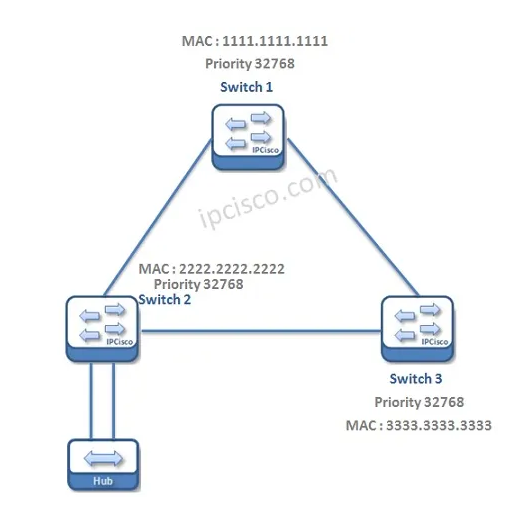
\includegraphics[width=0.7\linewidth]{screenshot002}
	\caption{}
	\label{fig:screenshot002}
\end{figure}

Aquí, se designará el puerto del puente raíz y el puerto de menor costo para el puente raíz en otros conmutadores será el puerto raíz.

En RSTP, se determinan dos puertos de bloqueo diferentes como mencionamos anteriormente. Aquí, el puerto de bloqueo en otro conmutador que no sea el puerto designado se seleccionará como puerto alternativo. Y el puerto de bloqueo en el mismo switch o segmento, será seleccionado como Puerto de Respaldo.
\begin{figure}[ph!]
	\centering
	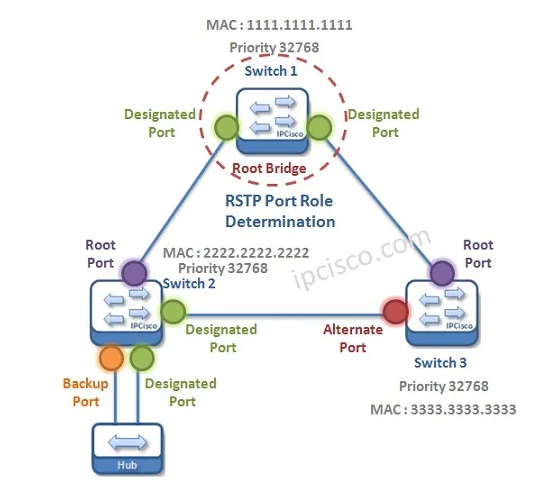
\includegraphics[width=0.7\linewidth]{screenshot003}
	\caption{}
	\label{fig:screenshot003}
\end{figure}


Interoperabilidad RSTP y STP
\\
Por último, mencionemos la interparabilidad de RSTP y STP. En diferentes redes, estos protocolos pueden funcionar juntos.

RSTP y STP son dos protocolos similares. En su red, puede haber conmutadores que admitan ambos protocolos de capa 2. Pero, ¿qué pasa si un conmutador de la red no admite RSTP? La respuesta es fácil. La topología LAyer 2 funciona únicamente con STP.
